\documentclass[10pt]{article}
\usepackage{enumerate}
\usepackage{tikz,tikz-cd,tikz-3dplot,pgfplots}
\usepackage{amsmath,amsthm,amssymb,amsfonts,amsthm}
\usepackage{hyperref}
\usepackage{mathrsfs}
\usepackage{bm,bbm}
\usepackage{braket}
\usepackage{slashed}
\usepackage{tensor}
\usepackage{caption, subcaption}
\usepackage{indentfirst}
\usepackage[a4paper, total={6.5in, 9in}]{geometry}
\usetikzlibrary{decorations.markings,positioning,decorations.pathmorphing}
\allowdisplaybreaks
\pgfplotsset{width=10cm, compat=1.16}
\renewcommand\bra[1]{{\langle{#1}|}}
\renewcommand\ket[1]{{|{#1}\rangle}}
\renewcommand\bfdefault{b}

\newtheorem{theorem}{Theorem}[section]
\newtheorem{lemma}[theorem]{Lemma}
\newtheorem{corollary}{Corollary}[theorem]
\theoremstyle{definition}
\newtheorem{definition}{Definition}[section]
\theoremstyle{remark}
\newtheorem{remark}{Remark}[section]

\DeclareMathOperator{\sech}{sech}
\DeclareMathOperator{\csch}{csch}
\DeclareMathOperator{\arcsec}{arcsec}
\DeclareMathOperator{\arccot}{arccot}
\DeclareMathOperator{\arccsc}{arccsc}
\DeclareMathOperator{\arccosh}{arccosh}
\DeclareMathOperator{\arcsinh}{arcsinh}
\DeclareMathOperator{\arctanh}{arctanh}
\DeclareMathOperator{\arcsech}{arcsech}
\DeclareMathOperator{\arccsch}{arccsch}
\DeclareMathOperator{\arccoth}{arccoth} 

\begin{document}
	\title{Hypothesis testing\\ \small How many samples do we need to verify threshold effects?}
	\maketitle
	\section{Assumptions}
	We examine the scattering of (almost) massless fermions, $\bar{f}f$.
	There can be three distinct kinds of events happening;
	No scattering $(\bar{f}f\to\bar{f}f)$, observable scattering $(\bar{f}f\to\Phi\to\bar{f}f)$, and decaying into the hidden or unknown sector $(\bar{f}f\to\Phi\to\bar{g}g)$.
	To simplify the argument, we combine the first and third events as background (B), and the second one is considered as a signal (S).
	Then the chance of getting signal is proportional to total cross section of the process $\bar{f}f\to\Phi\to\bar{f}f$.
	To further simplify the analysis, we will impose some assumptions:
	\begin{enumerate}
		\item A process in interest is dominant in $\bar{f}f$ scattering.
		That is, the contribution of other scattering processes are negligible.
		
		\item The detector classifies the background and the signal perfectly, which means that it does not confuse between no scattering events and observable scattering events.
		
		\item There is no systematic error or background noise.
		The only exception is the uncertainty of momentum measurement, which is dealt with binned counting or Gaussian smearing.
	\end{enumerate}
	In likelihood-ratio testing, we fix the mass of the hidden sector particle to prevent non-identifiability problem in Wilks' test\cite{algeri2020searching}.
	However, in practice we need to implement statistical corrections to prevent look-elsewhere effect.
	The other way around is using Pearson's $\chi^{2}$ test.
	It is convenient if we only need to reject the null hypothesis, but the drawback is that we cannot really tell much about the alternative models.
	
	It is impossible to predict the sample count needed without knowing the specific experimental procedure.
	In this report, I assumed that the invariant masses of the incoming particles are uniformly distributed along $M_{\mathrm{peak}}-2\Gamma_{\mathrm{tot}}<m_{\mathrm{in}}<M_{\mathrm{peak}}+2\Gamma_{\mathrm{tot}}$, where $M_{\mathrm{peak}}$ is the peak of resonance (real-on-shell mass) and $\Gamma_{\mathrm{tot}}$ is the total decay width of $\Phi$.
	
	\section{Likelihood-Ratio Test}
	\subsection{Unbinned Analysis without Momentum Uncertainties}
	If there are no uncertainties in momentum measurement, then we may perform the unbinned analysis.
	Suppose we got $N$ samples $x_{1},\dots,x_{N}$.
	For each sample $x_{i}$, $\mu_{i}=\mu(x_{i})$ is its invariant mass and $S(x_{i})$ is its measurement result, where $S(x_{i})=1$ if the detector counted it as a signal and $S(x_{i})=0$ for a background.
	
	The null hypothesis and the alternative hypothesis are
	\begin{align*}
		H_{0}&:P_{0}(\mu;A,M,\Gamma)=\frac{A\mu^{2}}{(\mu^{2}-M^{2})^{2}+\Gamma^{2}},\\
		H_{1}&:P_{1}(\mu;A,M,\Gamma,C\neq0)=\frac{A\mu^{2}}{|\mu^{2}-M^{2}+i\Gamma+C\Pi(\mu,m)|^{2}}.
	\end{align*}
	We can see that the alternative hypothesis has one extra degree of freedom in fitting parameters ($C$), since we have fixed $m$.
	
	Then the likelihood functions are given by
	\begin{align*}
		L_{0}(\theta)&=\prod_{i=1}^{N}\Big[S(x_{i})P_{0}(\mu_{i};\theta)+(1-S(x_{i}))(1-P_{0}(\mu_{i};\theta))\Big],\\
		L_{1}(\theta,C)&=\prod_{i=1}^{N}\Big[S(x_{i})P_{1}(\mu_{i};\theta,C)+(1-S(x_{i}))(1-P_{1}(\mu_{i};\theta,C))\Big].
	\end{align*}
	It is convenient to use log-likelihood functions instead:
	\begin{align*}
		\ln L_{0}(\theta)&=\sum_{i=1}^{N}\ln\Big[S(x_{i})P_{0}(\mu_{i};\theta)+(1-S(x_{i}))(1-P_{0}(\mu_{i};\theta))\Big],\\
		\ln L_{1}(\theta,C)&=\sum_{i=1}^{N}\ln\Big[S(x_{i})P_{1}(\mu_{i};\theta,C)+(1-S(x_{i}))(1-P_{1}(\mu_{i};\theta,C))\Big].
	\end{align*}
	The best fit is given by maximising likelihoods.
	
	Suppose that the alternative hypothesis is true:
	\[P(\mu)=P_{1}(\mu;\theta_{t},C_{t}),\quad C\neq0.\]
	Then the best fit parameters for $\theta$ and $C$ in the alternative hypothesis should be sufficiently close to the true values for big enough $N$.
	Hence, as $N\to\infty$,
	\begin{align*}
		\max_{\theta,C}\Big[\ln L_{1}(\theta,C)\Big]&\simeq\sum_{i=1}^{N}\ln\Big[S(x_{i})P(\mu_{i})+(1-S(x_{i}))(1-P(\mu_{i}))\Big]\\
		&\simeq\sum_{i=1}^{N}\Big[P(\mu_{i})\ln P(\mu_{i})+(1-P(\mu_{i}))\ln(1-P(\mu_{i}))\Big]\\
		&\simeq\frac{N}{4\Gamma_{\mathrm{tot}}}\int_{M_{t}-2\Gamma_{\mathrm{tot}}}^{M_{t}-2\Gamma_{\mathrm{tot}}}d\mu\,\Big[P(\mu)\ln P(\mu)+(1-P(\mu))\ln(1-P(\mu))\Big].
	\end{align*}
	The final quantity can be evaluated once we fix the true parameters.
	Similarly, for null hypothesis,
	\[\ln L_{0}(\theta)\simeq\frac{N}{4\Gamma_{\mathrm{tot}}}\int_{M_{t}-2\Gamma_{\mathrm{tot}}}^{M_{t}-2\Gamma_{\mathrm{tot}}}d\mu\,\Big[P(\mu)\ln P_{0}(\mu;\theta)+(1-P(\mu))\ln(1-P_{0}(\mu;\theta))\Big],\]
	so we can maximise $\ln L_{0}(\theta)$ with numerical computation.
	
	Once we have calculated $\mathcal{L}_{0}=\max_{\theta}[\ln L_{0}(\theta)]$ and $\mathcal{L}_{1}=\max_{\theta,C}[\ln L_{1}(\theta,C)]$, the log-likelihood-ratio
	\[t:=2\mathcal{L}_{1}-2\mathcal{L}_{0}\]
	is said to be following the $\chi^{2}(1)$ distribution.
	However, since the physically meaningful value of the extra parameter $C$ lies on the nonnegative half plane, our test statistics $t$ actually follows the $\frac{1}{2}\chi^{2}(1)$ distribution\cite{cowan2011asymptotic}.
	Then, if we want $5\sigma$ significance level, we should have $t>23.66$.
	Alternatively, since $t\propto N$, we can estimate the minimum sample number $N$ to get $5\sigma$ significance to reject the null hypothesis for given $P(\mu)$.
	
	Also, I found out that if $A$ is not so big (peak probability $\lesssim 10^{-2}$), $N$ is proportional to $A^{-1}$, which means that the total count of signal $N_{S}$ really matters.
	
	\subsection{Binned Analysis}
	To account for momentum uncertainties, we divide the range of $\mu$ into the bins with specific momentum ranges.
	Suppose that the range of $\mu$ of the $i$th bin is $\mu_{i;\mathrm{lower}}<\mu<\mu_{i;\mathrm{upper}}=\mu_{i;\mathrm{lower}}+\Delta\mu$.
	Then
	\begin{align*}
		H_{0}&:P_{0}(i;A,M,\Gamma)=\frac{1}{\Delta\mu}\int_{\mu_{i;\mathrm{lower}}}^{\mu_{i;\mathrm{upper}}}d\mu\,\frac{A\mu^{2}}{(\mu^{2}-M^{2})^{2}+\Gamma^{2}}=P_{0,i}(\theta),\\
		H_{1}&:P_{1}(i;A,M,\Gamma,C\neq0))=\frac{1}{\Delta\mu}\int_{\mu_{i;\mathrm{lower}}}^{\mu_{i;\mathrm{upper}}}d\mu\,\frac{A\mu^{2}}{|\mu^{2}-M^{2}+i\Gamma+C\Pi(\mu,m)|^{2}}=P_{1,i}(\theta,C).
	\end{align*}
	If there are in total $k$ bins, estimated log-likelihood functions are
	\begin{align*}
		\mathcal{L}_{0}&=\max_{\theta}\frac{N}{k}\sum_{i=1}^{k}\Big[P_{1,i}\ln P_{0,i}(\theta)+(1-P_{1,i})\ln(1-P_{0,i}(\theta))\Big],\\
		\mathcal{L}_{1}&=\frac{N}{k}\sum_{i=1}^{k}\Big[P_{1,i}\ln P_{1,i}+(1-P_{1,i})\ln(1-P_{1,i})\Big].
	\end{align*}
	
	\section{Result}
	Figure \ref{fig:unbinned} represents the required total signal counts for unbinned analysis.
	We can see that the discrepancy between Breit-Wigner distribution and the exact distribution could be easily detected when the mass of the loop particle is about the half of mass of the mother particle, and the coupling between mother particle and loop particle is strong.
	
	\begin{figure}[h]
		\centering
		\begin{subfigure}{0.3\textwidth}
			\centering
			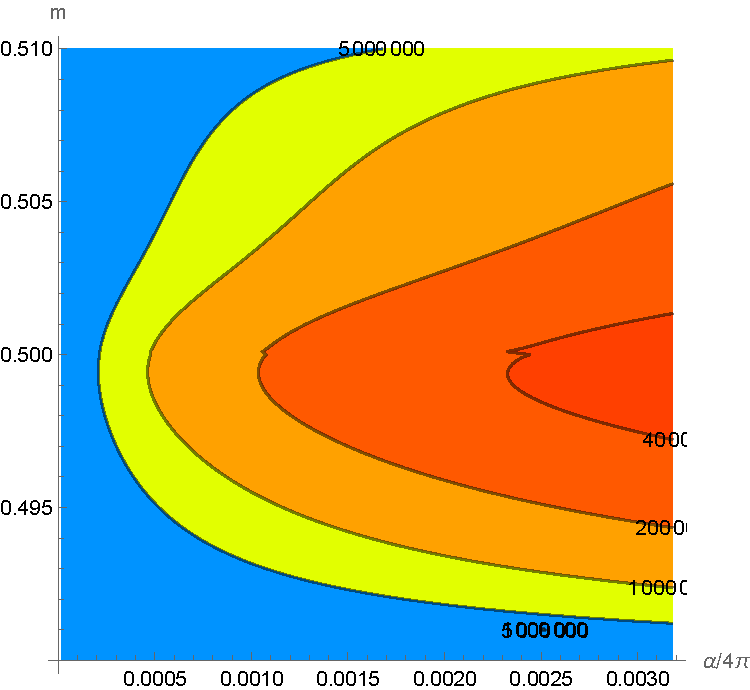
\includegraphics[width=\textwidth]{unbinned_0.01GeV.pdf}
			\caption{}
		\end{subfigure}
		\begin{subfigure}{0.3\textwidth}
			\centering
			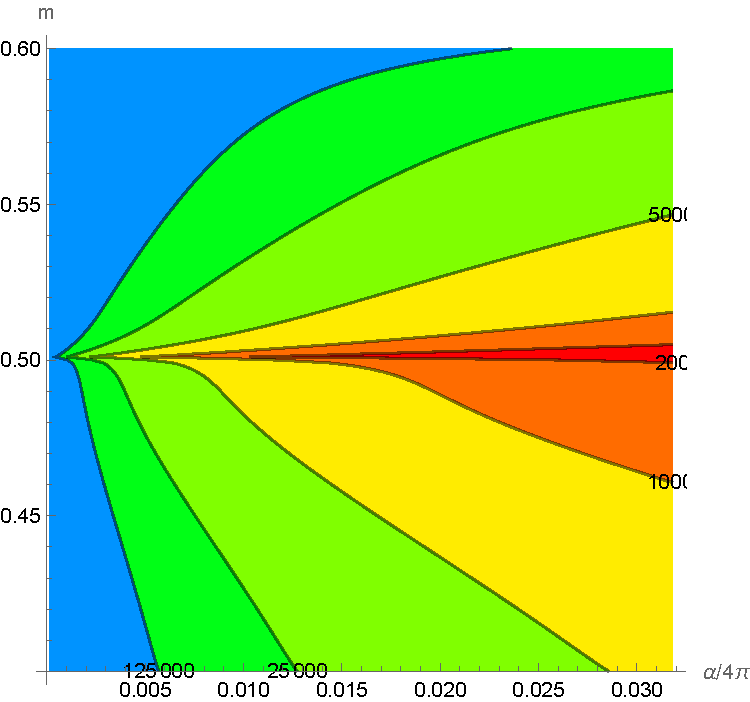
\includegraphics[width=\textwidth]{unbinned_0.1GeV.pdf}
			\caption{}
		\end{subfigure}
		\begin{subfigure}{0.3\textwidth}
			\centering
			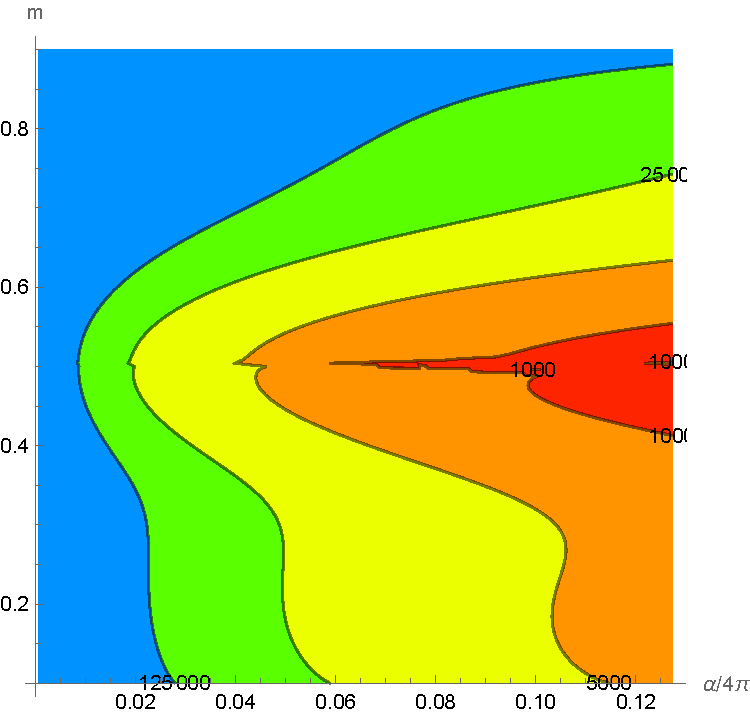
\includegraphics[width=\textwidth]{unbinned_0.4GeV.pdf}
			\caption{}
		\end{subfigure}
		\caption{Unbinned analysis result, with total width (a) $0.01\,\mathrm{GeV}$, (b) $0.1\,\mathrm{GeV}$, (c) $0.4\,\mathrm{GeV}$.}
		\label{fig:unbinned}
	\end{figure}
	
	Figure \ref{fig:binned} represents the required total signal counts for binned analysis, where each bin contains invariant mass interval whose length is $0.05\,\mathrm{GeV}$.
	
	\begin{figure}[h]
		\centering
		\begin{subfigure}{0.3\textwidth}
			\centering
			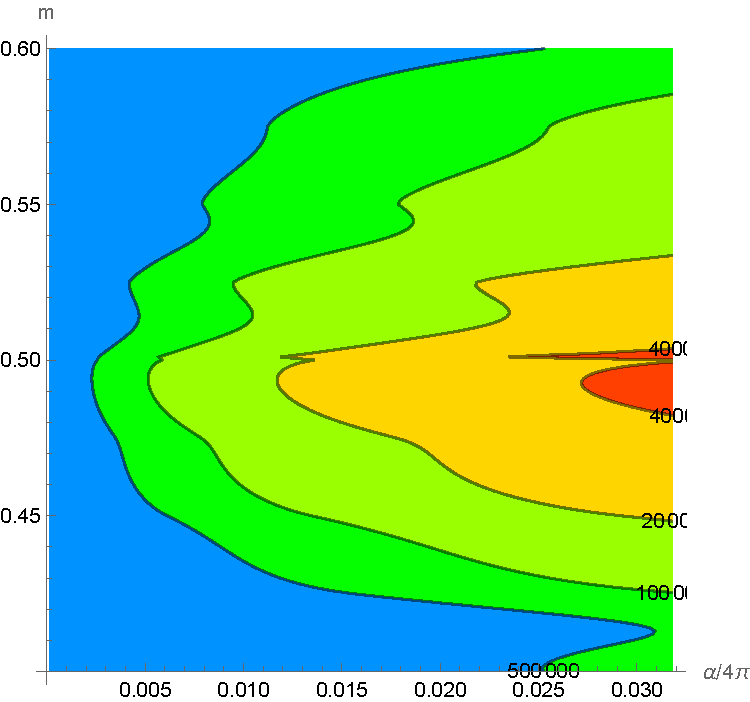
\includegraphics[width=\textwidth]{binned_0.1GeV.pdf}
			\caption{}
		\end{subfigure}
		\begin{subfigure}{0.3\textwidth}
			\centering
			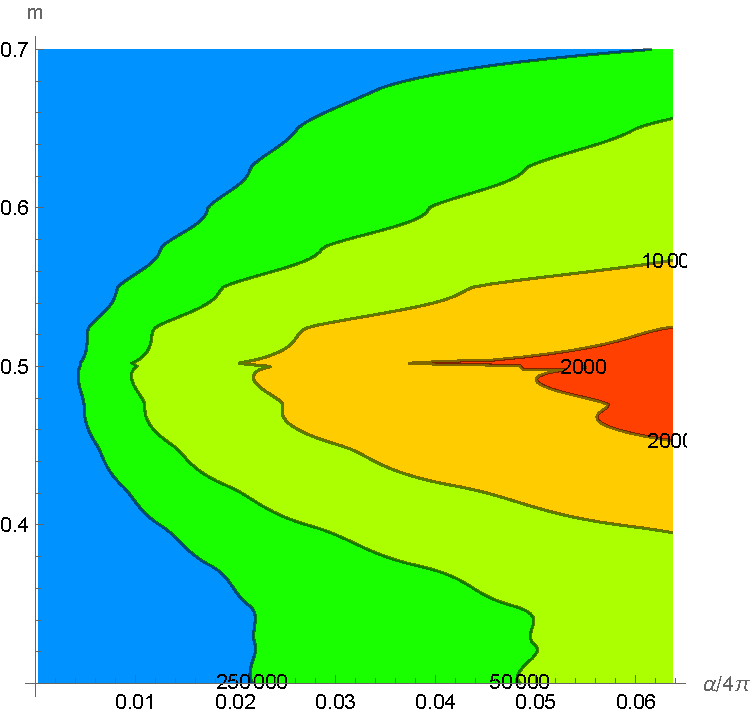
\includegraphics[width=\textwidth]{binned_0.2GeV.pdf}
			\caption{}
		\end{subfigure}
		\begin{subfigure}{0.3\textwidth}
			\centering
			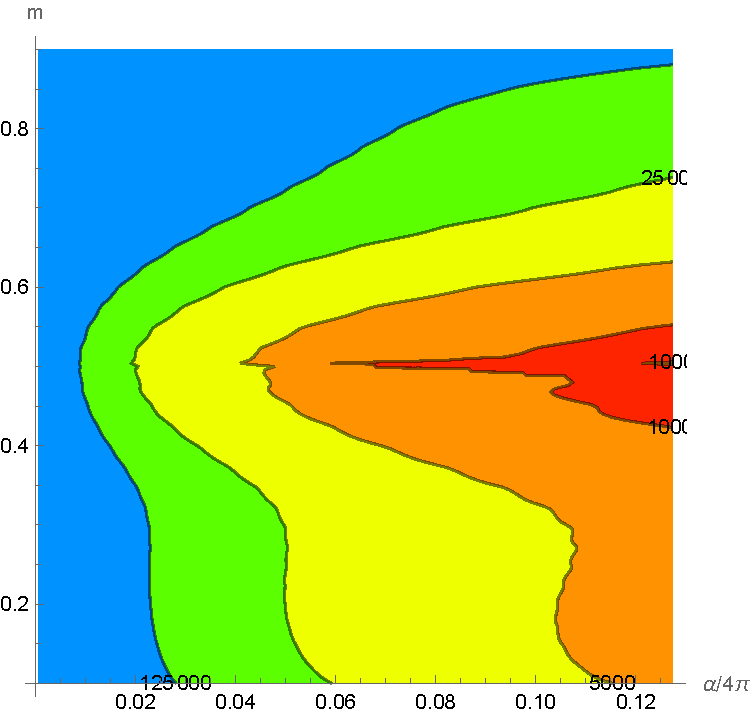
\includegraphics[width=\textwidth]{binned_0.4GeV.pdf}
			\caption{}
		\end{subfigure}
		\caption{Binned analysis result, with total width (a) $0.1\,\mathrm{GeV}$, (b) $0.2\,\mathrm{GeV}$, (c) $0.4\,\mathrm{GeV}$. Each bin's size is $0.05\,\mathrm{GeV}$.}
		\label{fig:binned}
	\end{figure}
	
	\bibliographystyle{unsrt}
	\bibliography{references}
\end{document}